\documentclass[]{article}
\usepackage{lmodern}
\usepackage{amssymb,amsmath}
\usepackage{graphicx}
\usepackage{ifxetex,ifluatex}
\usepackage{fixltx2e} % provides \textsubscript
\ifnum 0\ifxetex 1\fi\ifluatex 1\fi=0 % if pdftex
\usepackage[T1]{fontenc}
\usepackage[utf8]{inputenc}
\else % if luatex or xelatex
\ifxetex
\usepackage{mathspec}
\else
\usepackage{fontspec}
\fi
\defaultfontfeatures{Ligatures=TeX,Scale=MatchLowercase}
\fi
% use upquote if available, for straight quotes in verbatim environments
\IfFileExists{upquote.sty}{\usepackage{upquote}}{}
% use microtype if available
\IfFileExists{microtype.sty}{%
\usepackage{microtype}
\UseMicrotypeSet[protrusion]{basicmath} % disable protrusion for tt fonts
}{}
\usepackage[unicode=true]{hyperref}
\hypersetup{
pdfborder={0 0 0},
breaklinks=true}
\urlstyle{same}  % don't use monospace font for urls
\IfFileExists{parskip.sty}{%
\usepackage{parskip}
}{% else
\setlength{\parindent}{0pt}
\setlength{\parskip}{6pt plus 2pt minus 1pt}
}
\setlength{\emergencystretch}{3em}  % prevent overfull lines
\providecommand{\tightlist}{%
\setlength{\itemsep}{0pt}\setlength{\parskip}{0pt}}
\setcounter{secnumdepth}{0}
% Redefines (sub)paragraphs to behave more like sections
\ifx\paragraph\undefined\else
\let\oldparagraph\paragraph
\renewcommand{\paragraph}[1]{\oldparagraph{#1}\mbox{}}
\fi
\ifx\subparagraph\undefined\else
\let\oldsubparagraph\subparagraph
\renewcommand{\subparagraph}[1]{\oldsubparagraph{#1}\mbox{}}
\fi
\title{Specyfikacja implementacyjna programu JVac}
\date{}
\graphicspath{ {resources/} }

\begin{document}

    \maketitle

    \section{1 ) Kompilacja i uruchomienie}

    Program napisany został w Javie i wymaga maszyny wirtualnej tegoż języka
    (zalecana wersja: 11). Dodatkowo wykorzystywana jest biblioteka slf4j
    przy użyciu jdk14 do logowania. Przed pierwszym użyciem program powinien
    zostać skompilowany. W tym celu użytkownik powinien przejść do katalogu
    \emph{src/md/jvac} i wpisać następującą komendę

    \begin{center}
        \emph{javac JVac.java}
    \end{center}

    Program może zostać uruchomiony następującą komendą

    \begin{center}
        \emph{java JVac ŚCIEŻKA\_DO\_PLIKU\_WEJŚCIOWEGO}
    \end{center}


    \section{2 ) Struktura kodu źródłowego, opisy klas i pakietów}

    \begin{itemize}
        \item
        JVac -- Klasa sterująca działaniem programu (zawiera metodę main)
        \item
        md.jvac.simplex -- Pakiet odpowiedzialny za znalezienie optymalnego
        rozwiązania przy użyciu algorytmu sympleksowego

        \begin{itemize}
            \item
            SimplexSolver -- Klasa odpowiedzialna za przeprowadzenie algorytmu
            sympleksowego i zwrócenie końcowej tabeli sympleksowej
        \end{itemize}
        \item
        md.jvac.datastructures -- Pakiet zawierający klasy będące strukturami
        danych wykorzystywanymi przez program

        \begin{itemize}
            \item
            Matrix\textless{}T\textgreater{} - Klasa implementująca macierz

            \begin{itemize}
                \item
                SimplexTableau -- Macierz oparta na liczbach wymiernych,
                implementująca metody przydatne z punktu widzenia tabeli
                sympleksowej
            \end{itemize}
            \item
            TransactionSubject -- Klasa reprezentująca aptekę lub dostawcę
            \item
            Connection -- Klasa reprezentująca połączenie między apteką a
            dostawcą
            \item
            TransactionsData -- Klasa grupująca wszystkie dostępne apteki,
            dostawców i połączenia między nimi
            \item
            DataToTableauTransformer -- Klasa przerabiająca TransactionData na
            odpowiadającą jej SimplexTableau
        \end{itemize}
        \item
        md.jvac.rationalnumber -- Pakiet posiadający klasy potrzebne do
        implementacji liczb wymiernych

        \begin{itemize}
            \item
            RationalNumber\textless{}Comparable\textless{}RationalNumber\textgreater{}\textgreater{}
            -- Klasa reprezentująca liczbę wymierną
        \end{itemize}
        \item
        md.jvac.io -- Pakiet klas do obsługi wejścia i wyjścia

        \begin{itemize}
            \item
            InputFileReader -- Klasa służąca do odczytu pliku wejściowego i
            generacji obiektu klasy TransactionsData
            \item
            OutputFileWriter -- Klasa służąca do generacji pliku wyjściowego
            \item
            MessageCenter -- Klasa logująca poszczególne etapy algorytmu i
            ewentualnych wyjątków w programie
        \end{itemize}
        \item
        md.jvac.exceptions -- Pakiet niestandardowych wyjątków mogących
        występować w programie

        \begin{itemize}
            \item
            ImproperIndexingException -- Apteki lub producenci zostali
            poindeksowani w nierosnącej od 0 kolejności
            \item
            ImproperSectionHeaderException -- Nagłówek sekcji jest niepoprawny
            \item
            IllegalDailyProductionFormatException -- Dzienna produkcja nie jest
            liczbą lub nie jest dodatnią liczbą całkowitą
            \item
            IllegalDailyRequirementFormatException -- Dzienne zapotrzebowanie
            nie jest liczbą lub nie jest dodatnią liczbą całkowitą
            \item
            MissingConnectionException -- Istnieje apteka i producent między
            którymi nie ma połączenia
            \item
            IllegalDailyAvailabilityFormatException -- Dzienna dostępność
            szczepionek dla połączenia nie jest liczbą lub jest ujemną liczbą
            \item
            IllegalCostFormatException -- Koszt szczepionki nie jest liczbą lub
            nie jest liczbą dziesiętną z maksymalnie dwoma miejscami po
            przecinku
            \item
            IllegalDataStringException -- linijka danych pliku wejściowego jest
            niepoprawnie sformatowana (niepotrzebna białe znaki)
            \item
            TooManyTransactionSubjectsException -- Liczba aptek lub producentów
            przewyższa 1000
            \item
            DuplicatedTransactionSubjectNameException -- Powtarzające się nazwy
            producentów lub aptek
            \item
            ImproperSectionOrderException -- Sekcje nie są w poprawnej
            kolejności
        \end{itemize}
    \end{itemize}


    \section{3 ) Diagram UML}

    Uwaga: na diagramie oznaczono wyłącznie najważniejsze z punktu widzenia
    celu programu dane oraz metody.

    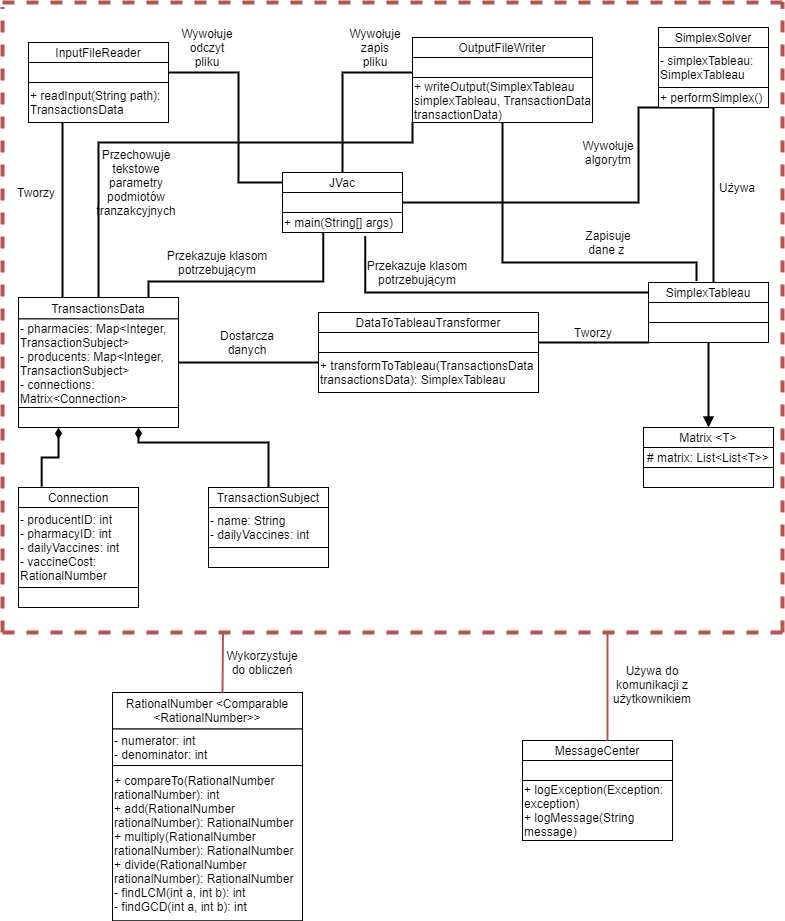
\includegraphics[scale=0.5]{UML}


    \section{4 ) Opis najważniejszych funkcji}

    \begin{itemize}
        \item
        main(String{[}{]} args) -- Steruje działaniem programu
        \item
        readInput(String path): TransactionsData -- Odczytuje zadany plik
        wejściowy i zwraca obiekt klasy TransactionsData na jego podstawie
        \item
        writeOutput(SimplexTableau simplexTableau, TransactionData
        transactionData)
        \item
        performSimplex() -- Tworzy plik wynikowy na podstawie danych
        wejściowych i znalezionego planu zakupu szczepionek
        \item
        transformToTableau(TransactionsData transactionsData): SimplexTableau
        -- Tworzy SimplexTableau na bazie zadanej struktury TransactionsData
        \item
        findLCM(int a, int b): int -- Znajduje NWW dwóch liczb
        \item
        findGCD(int a, int b): int -- Znajduje NWD dwóch liczb
        \item
        add/multipldivide(RationalNumber rationalNumber): RationalNumber --
        operacje na liczbach wymiernych
        \item
        logException(Exception: exception) -- Loguje zadany wyjątek
        \item
        logMessage(String message) -- Loguje zadaną wiadomość
    \end{itemize}


    \section{5 ) Diagram sekwencyjny programu}

    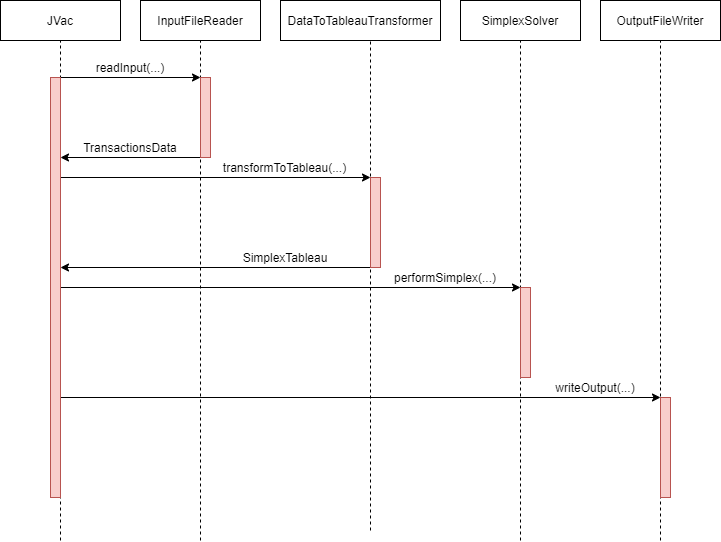
\includegraphics[scale=0.5]{StateDiagram}


    \section{6 ) Komunikacja z użytkownikiem}

    Dla każdego etapu programu (patrz: diagram sekwencyjny) program
    informuje o jego rozpoczęciu i zakończeniu. W przypadku konieczności
    zakończenia programu na skutek błędu/wyjątku jest on wyświetlany i
    dodatkowo opisywany użytkownikowi.

    \begin{flushright}
        \emph{Maciej Dragun\\*}
        \emph{298748 WE PW\\*}
        \emph{01142044@pw.edu.pl\\*}
    \end{flushright}

\end{document}

